\documentclass[12 pt]{amsart}
\usepackage{amsmath, amssymb, amsthm,amscd}
\usepackage{tkz-graph}
\usepackage{tikz}
\usepackage{tikz,fullpage}
\usetikzlibrary{positioning, quotes}
\usetikzlibrary{arrows,%
                petri,%
                topaths}%
\usetikzlibrary{graphs,quotes}
\usetikzlibrary{arrows,automata}
\usepackage[latin1]{inputenc}
\usepackage{tkz-berge}
\usepackage[position=top]{subfig}

\allowdisplaybreaks

\newcommand{\mathsym}[1]{{}}
\newcommand{\unicode}{{}}

\newtheorem{theorem}{Theorem}[section]
\newtheorem{lemma}[theorem]{Lemma}
\newtheorem{proposition}[theorem]{Proposition}
\newtheorem{corollary}[theorem]{Corollary}
\newtheorem{definition}[theorem]{Definition}
\newtheorem{construction}[theorem]{Construction}

\newcommand\T{\rule{0pt}{4.0ex}}       % Top strut
\newcommand\B{\rule[-2.5ex]{0pt}{0pt}} % Bottom strut

\newcommand{\smat}[4] {(\begin{smallmatrix} #1 & #2 \\ #3 & #4 \end{smallmatrix} )}
\newcommand{\mat}[4]  { \left(\begin{array}{cc} #1 & #2 \\ #3 & #4 \end{array} \right)}
\newcommand{\schar}[2] {( \begin{smallmatrix} #1 \\ #2 \end{smallmatrix})}

\newcommand{\op}[1]  { \operatorname{ #1 }}
\newcommand{\olbbH}[0]  { \overline{\mathbb{H}}}
\newcommand{\olbbQ}[0]  { \overline{\mathbb{Q}}}
\newcommand{\olG}[0]  { \overline{\Gamma}}
\newcommand{\bbH}[0]  { \mathbb{H}}
\newcommand{\bbC}[0]  { \mathbb{C}}
\newcommand{\bbZ}[0]  { \mathbb{Z}}
\newcommand{\bbF}[0]  { \mathbb{F}}
\newcommand{\bbQ}[0]  { \mathbb{Q}}
\newcommand{\bbR}[0]  { \mathbb{R}}
\newcommand{\gok}[0]  { \mathfrak{k}}
\newcommand{\goe}[0]  { \mathfrak{e}}
\newcommand{\goR}[0]  { \mathfrak{R}}



\addtolength{\textwidth}{1.0in}
\addtolength{\hoffset}{-0.5in}
\addtolength{\textheight}{0.0in}
\addtolength{\voffset}{-0.0in}

\begin{document}
\title{fft}

\section{fft/ifft}

\section{truncation}

Since zero-padding the input and output data to the next power of two obviously leads to performance jumps at powers of two, a \emph{truncated fft} is necessary, which assumes certain portions of the input and output are zero. If the convolution length is denoted by $n$ we expect
\begin{equation*}
\text{runtime} \sim n \log n\text{,}
\end{equation*}
so the more constant the ratio is, the better the truncation is working. Below is a plot of such a ratio when the input is further truncated to length $n/2$. which corresponds to assuming the top half of the $n$ inputs are zero. As expected, the truncated fft/ifft performs worst right after a power of two, but slightly unexpected is how bad the fft is there after $n>2^{23}$ and how well the ifft is there. There are performance bumps at $3 \cdot 2^n$, and, rather surprisingly, the non-truncated ifft is eventuallybeating the non-truncated fft by about $7\%$. This is surprising for the non-truncated version because they are performing the exact same calculations, just in a different order.

\begin{center}
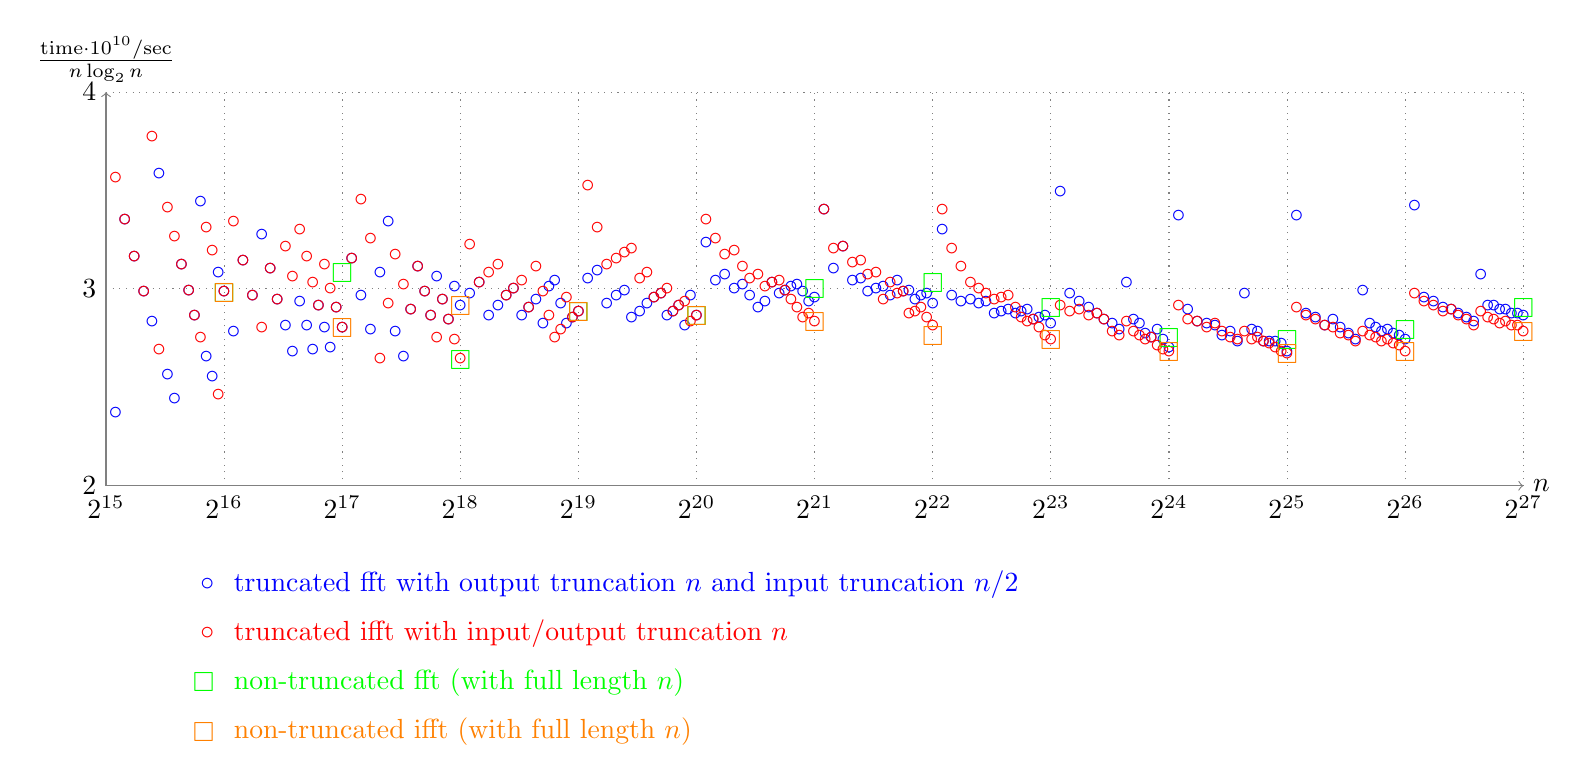
\begin{tikzpicture}[xscale=1.5, yscale=2.5]
\draw [dotted, gray] (15,2) grid (27,4);
\draw[latex-latex, thin, draw=gray, -to] (15,2)--(27,2) node [right] {$n$};
\draw[latex-latex, thin, draw=gray, -to] (15,2)--(15,4) node [above] {$\frac{\text{time} \cdot 10^{10}/\text{sec}}{n \log_2 n}$};

\foreach \Point in {2,3,4}{
    \node [black] at (15,\Point) [left] {$\Point$};
}

\foreach \Point in {15,16,...,27}{
    \node [black] at (\Point,2) [below] {$2^{\Point}$};
}

\foreach \Point in {(15.08,  2.37), (15.16,  3.35), (15.24,  3.16), (15.32,  2.98), (15.39,  2.83), (15.45,  3.58), (15.52,  2.56), (15.58,  2.44), (15.64,  3.12), (15.70,  2.99), (15.75,  2.86), (15.80,  3.44), (15.85,  2.65), (15.90,  2.55), (15.95,  3.08), (16.00,  2.98), (16.08,  2.78), (16.16,  3.14), (16.24,  2.96), (16.32,  3.27), (16.39,  3.10), (16.45,  2.94), (16.52,  2.81), (16.58,  2.68), (16.64,  2.93), (16.70,  2.81), (16.75,  2.69), (16.80,  2.91), (16.85,  2.80), (16.90,  2.70), (16.95,  2.90), (17.00,  2.80), (17.08,  3.15), (17.16,  2.96), (17.24,  2.79), (17.32,  3.08), (17.39,  3.34), (17.45,  2.78), (17.52,  2.65), (17.58,  2.89), (17.64,  3.11), (17.70,  2.98), (17.75,  2.86), (17.80,  3.06), (17.85,  2.94), (17.90,  2.84), (17.95,  3.01), (18.00,  2.91), (18.08,  2.97), (18.16,  3.03), (18.24,  2.86), (18.32,  2.91), (18.39,  2.96), (18.45,  3.00), (18.52,  2.86), (18.58,  2.90), (18.64,  2.94), (18.70,  2.82), (18.75,  3.01), (18.80,  3.04), (18.85,  2.92), (18.90,  2.82), (18.95,  2.85), (19.00,  2.88), (19.08,  3.05), (19.16,  3.09), (19.24,  2.92), (19.32,  2.96), (19.39,  2.99), (19.45,  2.85), (19.52,  2.88), (19.58,  2.92), (19.64,  2.95), (19.70,  2.97), (19.75,  2.86), (19.80,  2.88), (19.85,  2.91), (19.90,  2.81), (19.95,  2.96), (20.00,  2.86), (20.08,  3.23), (20.16,  3.04), (20.24,  3.07), (20.32,  3.00), (20.39,  3.02), (20.45,  2.96), (20.52,  2.90), (20.58,  2.93), (20.64,  3.03), (20.70,  2.97), (20.75,  2.99), (20.80,  3.01), (20.85,  3.02), (20.90,  2.98), (20.95,  2.93), (21.00,  2.95), (21.08,  3.40), (21.16,  3.10), (21.24,  3.21), (21.32,  3.04), (21.39,  3.05), (21.45,  2.98), (21.52,  3.00), (21.58,  3.01), (21.64,  2.96), (21.70,  3.04), (21.75,  2.98), (21.80,  2.99), (21.85,  2.94), (21.90,  2.96), (21.95,  2.97), (22.00,  2.92), (22.08,  3.30), (22.16,  2.96), (22.24,  2.93), (22.32,  2.94), (22.39,  2.92), (22.45,  2.93), (22.52,  2.87), (22.58,  2.88), (22.64,  2.89), (22.70,  2.87), (22.75,  2.88), (22.80,  2.89), (22.85,  2.84), (22.90,  2.85), (22.95,  2.86), (23.00,  2.82), (23.08,  3.49), (23.16,  2.97), (23.24,  2.93), (23.32,  2.90), (23.39,  2.87), (23.45,  2.84), (23.52,  2.82), (23.58,  2.79), (23.64,  3.03), (23.70,  2.84), (23.75,  2.82), (23.80,  2.77), (23.85,  2.75), (23.90,  2.79), (23.95,  2.74), (24.00,  2.70), (24.08,  3.37), (24.16,  2.89), (24.24,  2.83), (24.32,  2.82), (24.39,  2.81), (24.45,  2.76), (24.52,  2.78), (24.58,  2.73), (24.64,  2.97), (24.70,  2.79), (24.75,  2.78), (24.80,  2.73), (24.85,  2.73), (24.90,  2.73), (24.95,  2.72), (25.00,  2.68), (25.08,  3.37), (25.16,  2.87), (25.24,  2.85), (25.32,  2.81), (25.39,  2.84), (25.45,  2.80), (25.52,  2.77), (25.58,  2.74), (25.64,  2.99), (25.70,  2.82), (25.75,  2.80), (25.80,  2.78), (25.85,  2.79), (25.90,  2.77), (25.95,  2.76), (26.00,  2.74), (26.08,  3.42), (26.16,  2.95), (26.24,  2.93), (26.32,  2.90), (26.39,  2.89), (26.45,  2.87), (26.52,  2.85), (26.58,  2.83), (26.64,  3.07), (26.70,  2.91), (26.75,  2.91), (26.80,  2.89), (26.85,  2.89), (26.90,  2.87), (26.95,  2.87), (27.00,  2.86)}{
    \node [blue] at \Point {$\circ$};
}

\foreach \Point in {(15.08,  3.56), (15.16,  3.35), (15.24,  3.16), (15.32,  2.98), (15.39,  3.77), (15.45,  2.69), (15.52,  3.41), (15.58,  3.26), (15.64,  3.12), (15.70,  2.99), (15.75,  2.86), (15.80,  2.75), (15.85,  3.31), (15.90,  3.19), (15.95,  2.46), (16.00,  2.98), (16.08,  3.34), (16.16,  3.14), (16.24,  2.96), (16.32,  2.80), (16.39,  3.10), (16.45,  2.94), (16.52,  3.21), (16.58,  3.06), (16.64,  3.30), (16.70,  3.16), (16.75,  3.03), (16.80,  2.91), (16.85,  3.12), (16.90,  3.00), (16.95,  2.90), (17.00,  2.80), (17.08,  3.15), (17.16,  3.45), (17.24,  3.25), (17.32,  2.64), (17.39,  2.92), (17.45,  3.17), (17.52,  3.02), (17.58,  2.89), (17.64,  3.11), (17.70,  2.98), (17.75,  2.86), (17.80,  2.75), (17.85,  2.94), (17.90,  2.84), (17.95,  2.74), (18.00,  2.64), (18.08,  3.22), (18.16,  3.03), (18.24,  3.08), (18.32,  3.12), (18.39,  2.96), (18.45,  3.00), (18.52,  3.04), (18.58,  2.90), (18.64,  3.11), (18.70,  2.98), (18.75,  2.86), (18.80,  2.75), (18.85,  2.79), (18.90,  2.95), (18.95,  2.85), (19.00,  2.88), (19.08,  3.52), (19.16,  3.31), (19.24,  3.12), (19.32,  3.15), (19.39,  3.18), (19.45,  3.20), (19.52,  3.05), (19.58,  3.08), (19.64,  2.95), (19.70,  2.97), (19.75,  3.00), (19.80,  2.88), (19.85,  2.91), (19.90,  2.93), (19.95,  2.83), (20.00,  2.86), (20.08,  3.35), (20.16,  3.25), (20.24,  3.17), (20.32,  3.19), (20.39,  3.11), (20.45,  3.05), (20.52,  3.07), (20.58,  3.01), (20.64,  3.03), (20.70,  3.04), (20.75,  2.99), (20.80,  2.94), (20.85,  2.90), (20.90,  2.85), (20.95,  2.87), (21.00,  2.83), (21.08,  3.40), (21.16,  3.20), (21.24,  3.21), (21.32,  3.13), (21.39,  3.14), (21.45,  3.07), (21.52,  3.08), (21.58,  2.94), (21.64,  3.03), (21.70,  2.97), (21.75,  2.98), (21.80,  2.87), (21.85,  2.88), (21.90,  2.90), (21.95,  2.85), (22.00,  2.81), (22.08,  3.40), (22.16,  3.20), (22.24,  3.11), (22.32,  3.03), (22.39,  3.00), (22.45,  2.97), (22.52,  2.94), (22.58,  2.95), (22.64,  2.96), (22.70,  2.90), (22.75,  2.85), (22.80,  2.83), (22.85,  2.84), (22.90,  2.80), (22.95,  2.76), (23.00,  2.74), (23.08,  2.91), (23.16,  2.88), (23.24,  2.89), (23.32,  2.86), (23.39,  2.87), (23.45,  2.84), (23.52,  2.78), (23.58,  2.76), (23.64,  2.83), (23.70,  2.78), (23.75,  2.76), (23.80,  2.74), (23.85,  2.75), (23.90,  2.71), (23.95,  2.69), (24.00,  2.68), (24.08,  2.91), (24.16,  2.84), (24.24,  2.83), (24.32,  2.80), (24.39,  2.82), (24.45,  2.78), (24.52,  2.75), (24.58,  2.74), (24.64,  2.78), (24.70,  2.74), (24.75,  2.75), (24.80,  2.73), (24.85,  2.72), (24.90,  2.70), (24.95,  2.68), (25.00,  2.67), (25.08,  2.90), (25.16,  2.86), (25.24,  2.84), (25.32,  2.81), (25.39,  2.80), (25.45,  2.77), (25.52,  2.76), (25.58,  2.73), (25.64,  2.78), (25.70,  2.76), (25.75,  2.75), (25.80,  2.73), (25.85,  2.74), (25.90,  2.72), (25.95,  2.71), (26.00,  2.68), (26.08,  2.97), (26.16,  2.93), (26.24,  2.91), (26.32,  2.88), (26.39,  2.89), (26.45,  2.86), (26.52,  2.84), (26.58,  2.81), (26.64,  2.88), (26.70,  2.85), (26.75,  2.84), (26.80,  2.82), (26.85,  2.83), (26.90,  2.81), (26.95,  2.81), (27.00,  2.78)}{
    \node [red] at \Point {$\circ$};
}

\foreach \Point in {(16.00,  2.98), (17.00,  3.08), (18.00,  2.64), (19.00,  2.88), (20.00,  2.86), (21.00,  3.00), (22.00,  3.03), (23.00,  2.90), (24.00,  2.75), (25.00,  2.74), (26.00,  2.79), (27.00,  2.90)}{
    \node [green] at \Point {$\square$};
}

\foreach \Point in {(16.00,  2.98), (17.00,  2.80), (18.00,  2.91), (19.00,  2.88), (20.00,  2.86), (21.00,  2.83), (22.00,  2.76), (23.00,  2.74), (24.00,  2.68), (25.00,  2.67), (26.00,  2.68), (27.00,  2.78)}{
    \node [orange] at \Point {$\square$};
}


\node [blue] at (16,1.5) [left] {$\circ$};
\node [blue] at (16,1.5) [right] {truncated fft with output truncation $n$ and input truncation $n/2$};

\node [red] at (16,1.25) [left] {$\circ$};
\node [red] at (16,1.25) [right] {truncated ifft with input/output truncation $n$};

\node [green] at (16,1.0) [left] {$\square$};
\node [green] at (16,1.0) [right] {non-truncated fft (with full length $n$)};

\node [orange] at (16,0.75) [left] {$\square$};
\node [orange] at (16,0.75) [right] {non-truncated ifft (with full length $n$)};

\end{tikzpicture}
\end{center}


\newpage

Same picture for \texttt{\{i\}fft\_mfa\_truncate\_sqrt2} with $2^{16}$ bit coefficients to support the final long convolution length of $2^{18}$.


\begin{center}
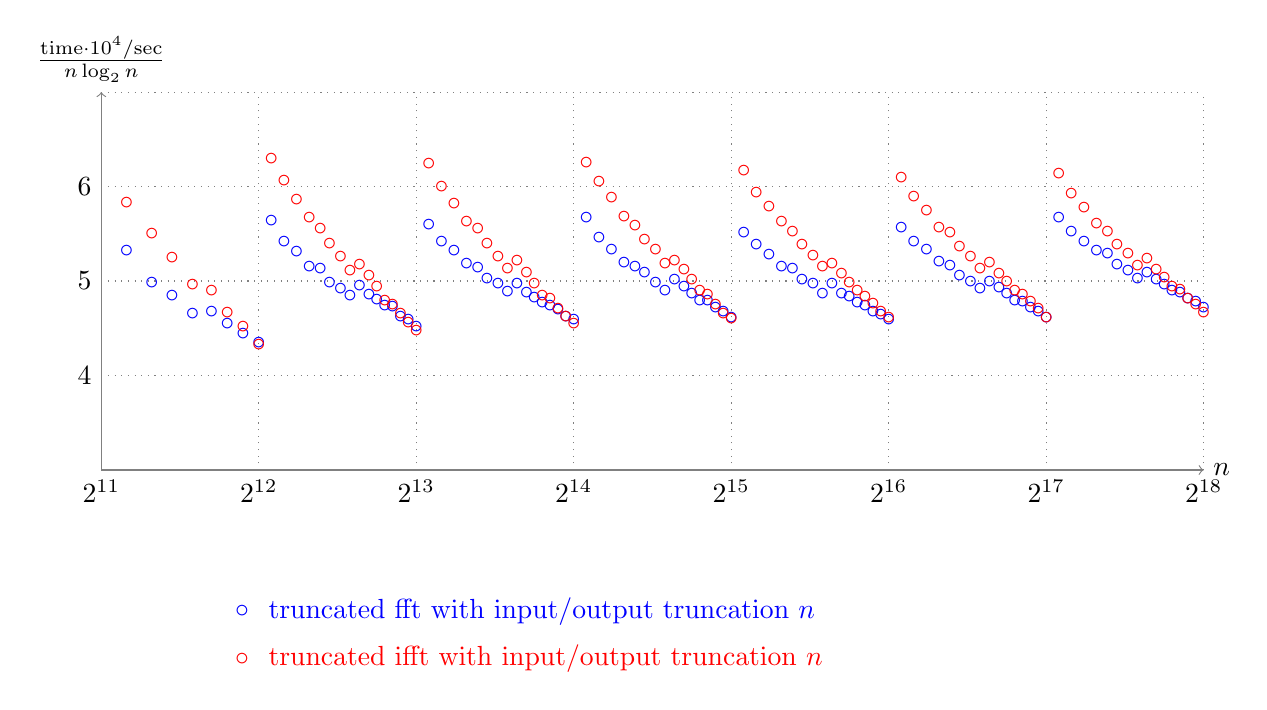
\begin{tikzpicture}[xscale=2.0, yscale=1.2]
\draw [dotted, gray] (11,3) grid (18,7);
\draw[latex-latex, thin, draw=gray, -to] (11,3)--(18,3) node [right] {$n$};
\draw[latex-latex, thin, draw=gray, -to] (11,3)--(11,7) node [above] {$\frac{\text{time} \cdot 10^{4}/\text{sec}}{n \log_2 n}$};

\foreach \Point in {4,5,6}{
    \node [black] at (11,\Point) [left] {$\Point$};
}

\foreach \Point in {11,12,...,18}{
    \node [black] at (\Point,3) [below] {$2^{\Point}$};
}

\foreach \Point in {(11.16,  5.31), (11.32,  4.98), (11.45,  4.84), (11.58,  4.65), (11.70,  4.67), (11.80,  4.54), (11.90,  4.44), (12.00,  4.34), (12.08,  5.63), (12.16,  5.41), (12.24,  5.30), (12.32,  5.15), (12.39,  5.12), (12.45,  4.98), (12.52,  4.91), (12.58,  4.84), (12.64,  4.94), (12.70,  4.85), (12.75,  4.80), (12.80,  4.73), (12.85,  4.72), (12.90,  4.62), (12.95,  4.58), (13.00,  4.51), (13.08,  5.59), (13.16,  5.41), (13.24,  5.31), (13.32,  5.18), (13.39,  5.13), (13.45,  5.02), (13.52,  4.97), (13.58,  4.88), (13.64,  4.96), (13.70,  4.87), (13.75,  4.82), (13.80,  4.76), (13.85,  4.73), (13.90,  4.69), (13.95,  4.62), (14.00,  4.58), (14.08,  5.66), (14.16,  5.45), (14.24,  5.32), (14.32,  5.19), (14.39,  5.15), (14.45,  5.08), (14.52,  4.98), (14.58,  4.89), (14.64,  5.01), (14.70,  4.93), (14.75,  4.86), (14.80,  4.79), (14.85,  4.78), (14.90,  4.71), (14.95,  4.67), (15.00,  4.60), (15.08,  5.50), (15.16,  5.38), (15.24,  5.27), (15.32,  5.14), (15.39,  5.12), (15.45,  5.01), (15.52,  4.96), (15.58,  4.86), (15.64,  4.96), (15.70,  4.86), (15.75,  4.83), (15.80,  4.76), (15.85,  4.73), (15.90,  4.67), (15.95,  4.64), (16.00,  4.58), (16.08,  5.56), (16.16,  5.41), (16.24,  5.32), (16.32,  5.20), (16.39,  5.16), (16.45,  5.05), (16.52,  4.99), (16.58,  4.91), (16.64,  4.99), (16.70,  4.92), (16.75,  4.86), (16.80,  4.79), (16.85,  4.77), (16.90,  4.71), (16.95,  4.67), (17.00,  4.61), (17.08,  5.66), (17.16,  5.52), (17.24,  5.41), (17.32,  5.31), (17.39,  5.28), (17.45,  5.17), (17.52,  5.10), (17.58,  5.02), (17.64,  5.08), (17.70,  5.01), (17.75,  4.95), (17.80,  4.89), (17.85,  4.87), (17.90,  4.81), (17.95,  4.77), (18.00,  4.71)}{
    \node [blue] at \Point {$\circ$};
}

\foreach \Point in {(11.16,  5.82), (11.32,  5.49), (11.45,  5.24), (11.58,  4.95), (11.70,  4.89), (11.80,  4.66), (11.90,  4.51), (12.00,  4.32), (12.08,  6.29), (12.16,  6.06), (12.24,  5.85), (12.32,  5.66), (12.39,  5.55), (12.45,  5.39), (12.52,  5.25), (12.58,  5.10), (12.64,  5.17), (12.70,  5.05), (12.75,  4.93), (12.80,  4.79), (12.85,  4.74), (12.90,  4.65), (12.95,  4.55), (13.00,  4.47), (13.08,  6.23), (13.16,  5.99), (13.24,  5.81), (13.32,  5.62), (13.39,  5.55), (13.45,  5.39), (13.52,  5.25), (13.58,  5.12), (13.64,  5.21), (13.70,  5.08), (13.75,  4.96), (13.80,  4.84), (13.85,  4.81), (13.90,  4.70), (13.95,  4.62), (14.00,  4.54), (14.08,  6.25), (14.16,  6.04), (14.24,  5.88), (14.32,  5.67), (14.39,  5.58), (14.45,  5.43), (14.52,  5.32), (14.58,  5.18), (14.64,  5.21), (14.70,  5.11), (14.75,  5.01), (14.80,  4.89), (14.85,  4.85), (14.90,  4.74), (14.95,  4.65), (15.00,  4.59), (15.08,  6.16), (15.16,  5.93), (15.24,  5.78), (15.32,  5.62), (15.39,  5.52), (15.45,  5.38), (15.52,  5.26), (15.58,  5.15), (15.64,  5.18), (15.70,  5.07), (15.75,  4.98), (15.80,  4.89), (15.85,  4.83), (15.90,  4.75), (15.95,  4.67), (16.00,  4.60), (16.08,  6.09), (16.16,  5.89), (16.24,  5.74), (16.32,  5.56), (16.39,  5.50), (16.45,  5.36), (16.52,  5.25), (16.58,  5.12), (16.64,  5.19), (16.70,  5.07), (16.75,  4.99), (16.80,  4.89), (16.85,  4.85), (16.90,  4.77), (16.95,  4.70), (17.00,  4.61), (17.08,  6.13), (17.16,  5.92), (17.24,  5.77), (17.32,  5.60), (17.39,  5.52), (17.45,  5.38), (17.52,  5.28), (17.58,  5.16), (17.64,  5.23), (17.70,  5.11), (17.75,  5.03), (17.80,  4.93), (17.85,  4.90), (17.90,  4.81), (17.95,  4.74), (18.00,  4.66)}{
    \node [red] at \Point {$\circ$};
}


\node [blue] at (12,1.5) [left] {$\circ$};
\node [blue] at (12,1.5) [right] {truncated fft with input/output truncation $n$};

\node [red] at (12,1.0) [left] {$\circ$};
\node [red] at (12,1.0) [right] {truncated ifft with input/output truncation $n$};


\end{tikzpicture}
\end{center}




\end{document}

